% !TEX root = ../main.tex
\section{Theoretical basis}

\begin{frame}{Theoretical basis}
    \begin{block}{Convolution }
      \textbf{Convolution} provides a way of `multiplying together' two arrays of numbers, generally of different sizes, but of the same dimensionality, to produce a third array of numbers of the same dimensionality\autocite{mlcb}.
    \end{block}
    \begin{columns}
      \begin{column}{0.5\textwidth}
        The convolution is performed by sliding the kernel over the image, generally starting at the top left corner, so as to move the kernel through all the positions where the kernel fits entirely within the boundaries of the image. Each kernel position corresponds to a single output pixel, the value of which is calculated by multiplying together the kernel value and the underlying image pixel value for each of the cells in the kernel, and then adding all these numbers together.
      \end{column}
      \begin{column}{0.5\textwidth}
        \begin{figure}
          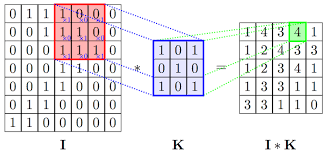
\includegraphics[width=\textwidth]{figure/conv2d.png}
          \caption{Convolution}
        \end{figure}
      \end{column}
    \end{columns}
\end{frame}

\begin{frame}{Theoretical basis}
  \begin{block}{1D Convolution}
    \textbf{1D Convolution} is a sort of convolution which is for signals or speech.
  \end{block}
  \begin{figure}
    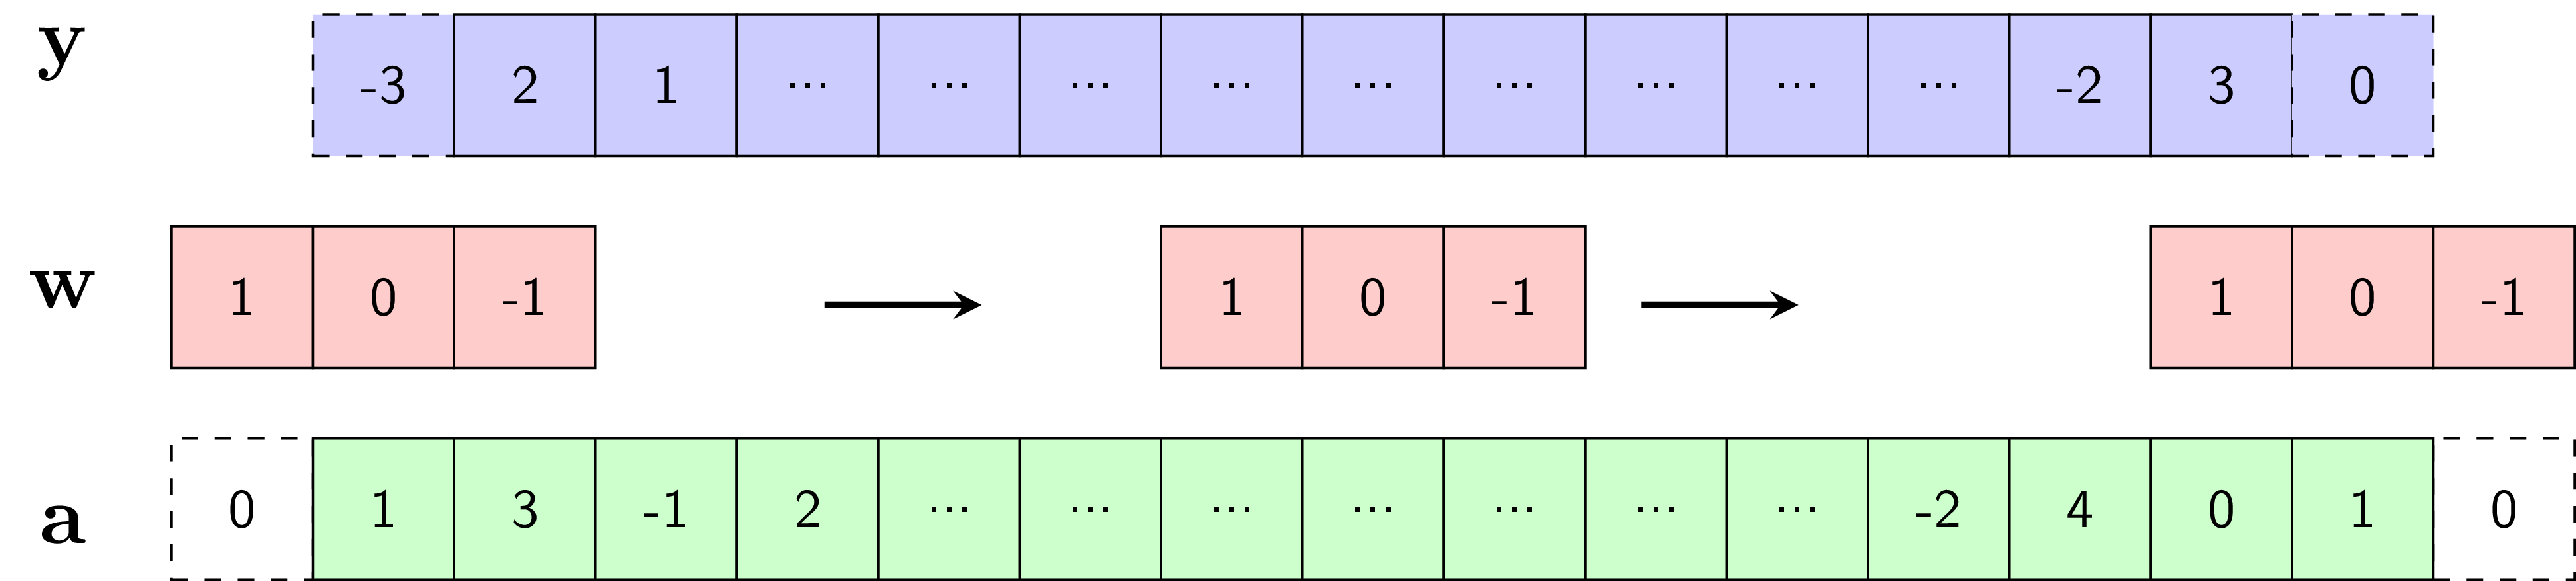
\includegraphics[width=\textwidth]{figure/conv1d_padding.png}
    \caption{1D Convolution}
  \end{figure}
\end{frame}

\begin{frame}{Theoretical basis}
  \begin{block}{Pooling layer}
    \textbf{Pooling} is the process of extracting the features from the image output of a convolution layer. This will also follow the same process of sliding over the image with a specified pool size/kernel size.
  \end{block}
  \begin{columns}
    \begin{column}{0.6\textwidth}
      There are two types of pooling is available:
      \begin{enumerate}
        \item Max Pooling
        \item Average Pooling
      \end{enumerate}
      Max Pooling is being used widely and it will just keep the highest number in the pool and discard the rest. By getting the highest value in each pool we will be getting the significant features of the image, the lower values are not the features at all or not significant features to be able to use in the model.
    \end{column}
    \begin{column}{0.4\textwidth}
      \begin{figure}
        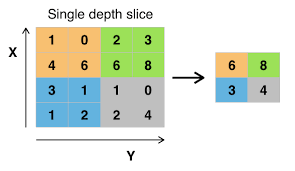
\includegraphics[width=\textwidth]{figure/pooling.png}
        \caption{Example of Max Pooling}
      \end{figure}
    \end{column}
  \end{columns}
\end{frame}

\begin{frame}{Theoretical basis}
  \begin{block}{Batch Normalizing Transform}
  \textbf{Batch normalization (or batch norm)} is a method used to make NNnet faster and more stable through normalization of the layer's inputs by re-centrering and re-scaling.

  Use B to denote a mini-batch of size m of the entire training set. The empirical \textbf{mean} and \textbf{variance} of B could thus be denoted as:
  \begin{equation}
    \mu = \frac{1}{m}\sum_{i=1}^{m}{x_i}\ ; \sigma^2 = \frac{1}{m}\sigma_{i=1}^{m}{(x_i-\mu_B)^2}
  \end{equation}

  For a layer of the network with d-dimensional input \(x = (x^{(1)},..., x^{(d)})\), each dimension of its input is then normalized (i.e. recentered and re-scaled) separately.
  \begin{equation}
    \hat{x}^{(k)} = \frac{x_i^{(k)} - \mu_B^{(k)}}{\sqrt{\sigma_b^{(k)^2} + \epsilon}}
  \end{equation}
  where \(k \in [1,d]\); \(i \in [1,m]\) and \(\mu_B^{(k)}\), \(\sigma_B^{(k)^2}\) are the per-dimension mean and variance, respectively.
  \end{block}
\end{frame}

\begin{frame}{Theoretical basis}
  \begin{block}{Softmax function}
    \textbf{The softmax function} is a generalization of the logistic function to multiple dimensions. It is used in multinomial logistic regression and is often used as the last activation function of a neural network to normalize the output of a network to a probability distribution over predicted output classes.

    The softmax function takes as input a vector z of K real numbers, and normalizes it into a probability distribution consisting of K probabilities proportional to the exponentials of the input numbers.

    The standard (unit) softmax function \(\sigma:\mathbb{R}^K \rightarrow\ [0,1]^K\) is defined by the formula:
    \begin{equation}
      \sigma(z)_i = \frac{e^{z_i}}{\sum_{j=1}^K{e^{z_j}}}\ \text{for}\ i=1,...,K \ \text{and}\ z = (z_1,...,z_K) \in \mathbb{R}^K
    \end{equation}
  \end{block}
\end{frame}
